\documentclass{article}
\usepackage[T1]{fontenc}
\usepackage{fancyhdr}
\usepackage{extramarks}
\usepackage{amsmath}
\usepackage{amsthm}
\usepackage{amsfonts}
\usepackage{dsfont}
\usepackage{tikz}
\usepackage[plain]{algorithm}
\usepackage{algpseudocode}
\usepackage{graphicx}
\usepackage{listings}
\usepackage{enumitem}

\graphicspath{ {./../img} }

\usetikzlibrary{automata,positioning}

%
% Basic Document Settings
%

\topmargin=-0.45in
\evensidemargin=0in
\oddsidemargin=0in
\textwidth=6.5in
\textheight=9.0in
\headsep=0.25in

\linespread{1.1}

\pagestyle{fancy}
\lhead{\hmwkAuthorName}
\chead{\hmwkTitle}
\rhead{\hmwkClass}
\lfoot{\lastxmark}
\cfoot{\thepage}

\renewcommand\headrulewidth{0.4pt}
\renewcommand\footrulewidth{0.4pt}

\setlength\parindent{0pt}
\setlength{\parskip}{5pt}

%
% Homework Details
%   - Title
%   - Due date
%   - Class
%   - Section/Time
%   - Instructor
%   - Author
%

\newcommand{\hmwkTitle}{Quiz\ \#3}
\newcommand{\hmwkDueDate}{November 27, 2023}
\newcommand{\hmwkClass}{ECE 271A}
\newcommand{\hmwkClassInstructor}{Professor Vasconcelos}
\newcommand{\hmwkAuthorName}{\textbf{Ray Tsai}}
\newcommand{\hmwkPID}{A16848188}

%
% Title Page
%

\title{
    \vspace{2in}
    \textmd{\textbf{\hmwkClass:\ \hmwkTitle}}\\
    \normalsize\vspace{0.1in}\small{Due\ on\ \hmwkDueDate\ at 11:59pm}\\
    \vspace{0.1in}\large{\textit{\hmwkClassInstructor}} \\
    \vspace{3in}
}

\author{
  \hmwkAuthorName \\
  \vspace{0.1in}\small\hmwkPID
}
\date{}

%
% Various Helper Commands
%

% Useful for algorithms
\newcommand{\alg}[1]{\textsc{\bfseries \footnotesize #1}}

% For derivatives
\newcommand{\deriv}[1]{\frac{\mathrm{d}}{\mathrm{d}x} (#1)}

% For partial derivatives
\newcommand{\pderiv}[2]{\frac{\partial}{\partial #1} (#2)}

% Integral dx
\newcommand{\dx}{\mathrm{d}x}

% Probability commands: Expectation, Variance, Covariance, Bias
\newcommand{\Var}{\mathrm{Var}}
\newcommand{\Cov}{\mathrm{Cov}}
\newcommand{\Bias}{\mathrm{Bias}}
\newcommand*{\Z}{\mathbb{Z}}
\newcommand*{\Q}{\mathbb{Q}}
\newcommand*{\R}{\mathbb{R}}
\newcommand*{\C}{\mathbb{C}}
\newcommand*{\N}{\mathbb{N}}
\newcommand*{\prob}{\mathds{P}}
\newcommand*{\E}{\mathds{E}}
\newcommand*{\G}{\mathcal{G}}
\newcommand*{\D}{\mathcal{D}}

\begin{document}

\maketitle

\pagebreak

\section*{Parameters}

We assume that the class-conditional,
\[
    P_{\mathbf{x}|\mu, \mathbf{\Sigma}} = \G(\mathbf{x}, \mu, \mathbf{\Sigma}),
\]
where
\[
    \mathbf{\Sigma} = \frac{1}{N}\sum_{i = 1}^N \left(x_i - \frac{1}{N}\sum_{k = 1}^N \mathbf{x}_k\right)\left(x_i - \frac{1}{N}\sum_{i = k}^N \mathbf{x}_k\right)^T,
\]
is the covariance matrix of the sample and $\mu$ is a random variable of the distribution
\[
    P_{\mu}(\mu) = \G(\mu, \mu_0, \mathbf{\Sigma}_0),
\]
with $\mathbf{\Sigma}_0 = diag(\alpha\mathbf{w})$, for $\mathbf{w}$ and $\mu_0$ given from the dataset.

\subsection*{Predictive Distribution}

For each class $i$, we compute the parameters of
\[
    P_{\mu|\mathbf{T}}(\mu | \D_i) = \G(\mu, \mu_i, \mathbf{\Sigma}_i).
\]
From the textbook, we know
\begin{gather*}
    \mu_i = \mathbf{\Sigma}_0\left(\mathbf{\Sigma}_0 + \frac{1}{N}\mathbf{\Sigma}\right)^{-1}\mu_{sample} + \frac{1}{N}\mathbf{\Sigma}\left(\mathbf{\Sigma}_0 + \frac{1}{N}\mathbf{\Sigma}\right)^{-1}\mu_0, \\
    \mathbf{\Sigma}_i = \mathbf{\Sigma}_0\left(\mathbf{\Sigma}_0 + \frac{1}{N}\mathbf{\Sigma}\right)^{-1}\frac{1}{N}\mathbf{\Sigma},
\end{gather*}
where $\mu_{sample} = \frac{1}{N}\sum_{i = 1}^N \mathbf{x}_i$.
This immediately follows that the predictive distribution
\[
    P_{\mathbf{x}|\mathbf{T}}(\mathbf{x}|\D_i) = \G(\mathbf{x}, \mu_i, \mathbf{\Sigma} + \mathbf{\Sigma}_i).
\]

\subsection*{Maximum Likelihood Estimate}

The maximum likelihood estimate of the class conditional distribution is
\[
    P_{\mathbf{x}|\mathbf{T}}(\mathbf{x}|\D_i) = \G(\mathbf{x}, \mu_{sample}, \mathbf{\Sigma}).
\]

\subsection*{MAP Approximation}

The MAP approximation of the posterior mean is simply the posterior mean we obtained above. Thus,
\[
    P_{\mathbf{x}|\mathbf{T}}(\mathbf{x}|\D_i) = \G(\mathbf{x}, \mu_{i}, \mathbf{\Sigma}).
\]

\pagebreak

\section*{Curves}

\begin{center}
    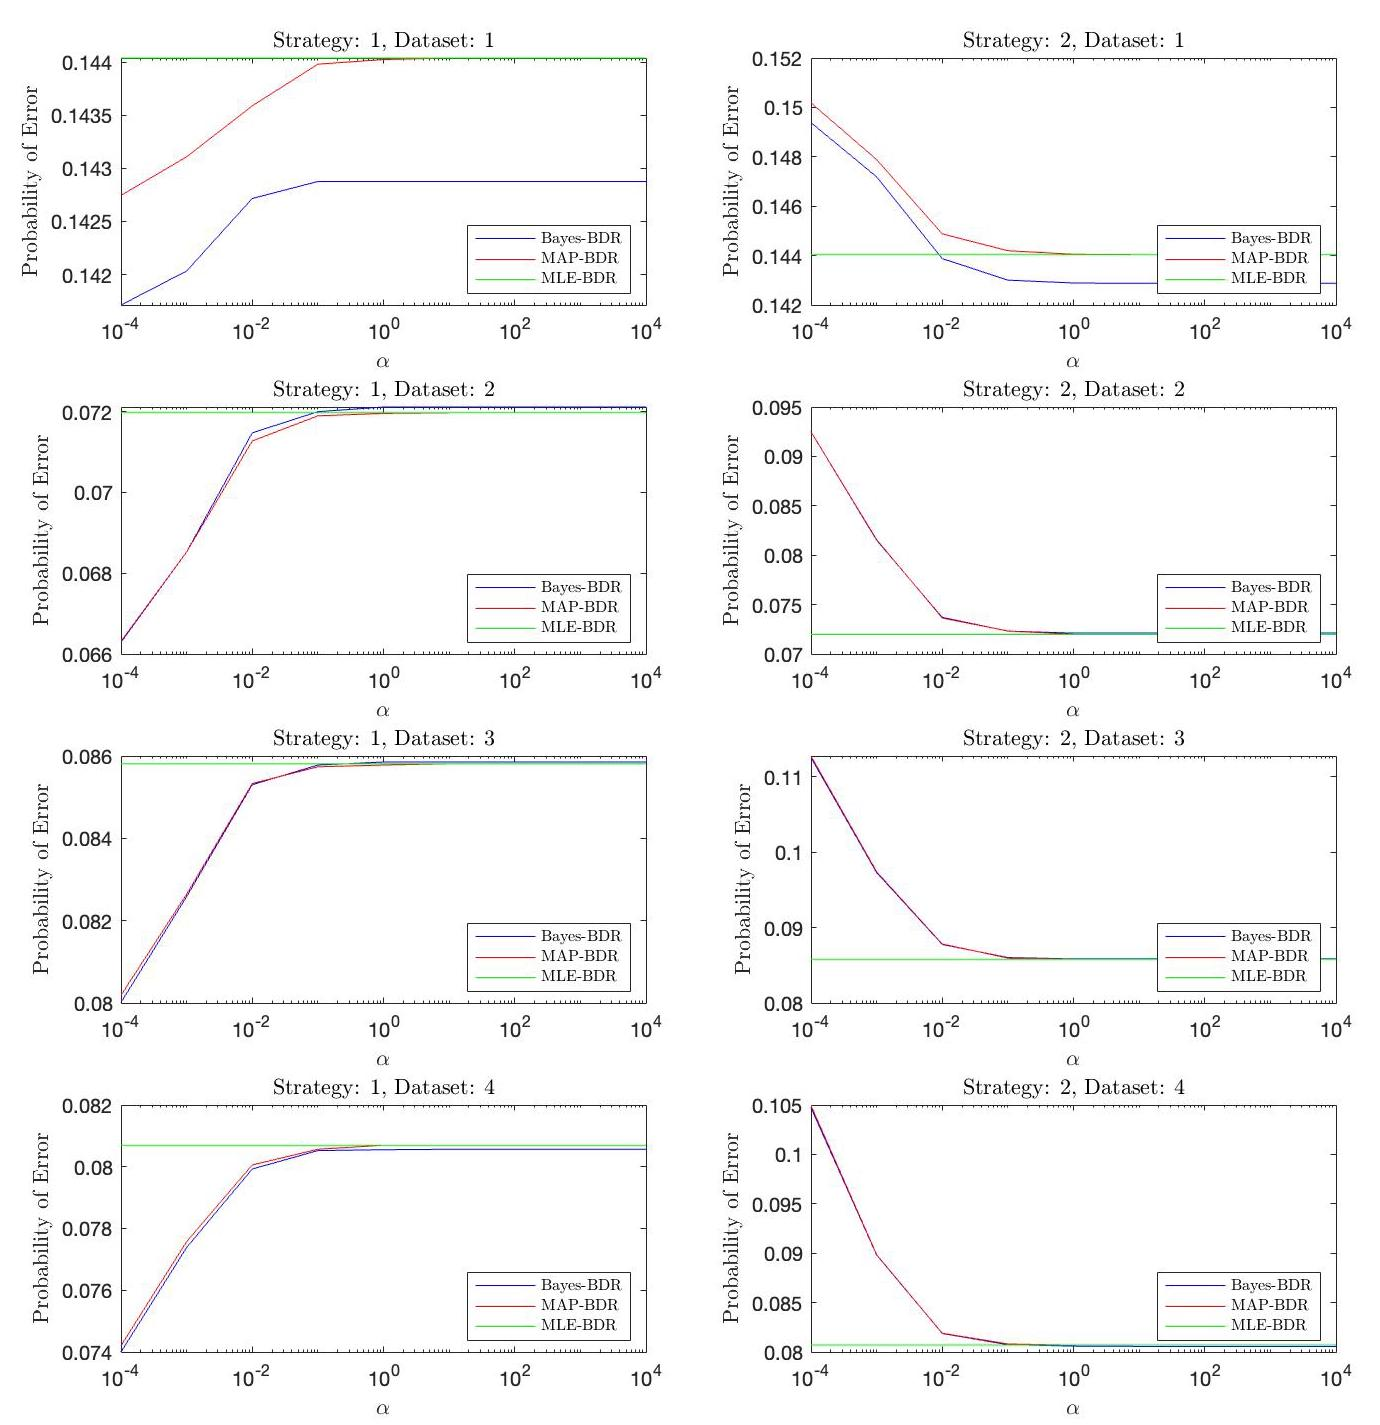
\includegraphics[width=\textwidth]{poe}
\end{center}

\pagebreak

\section*{Interpretations}

\subsection*{Part A}

We examine the Bayes plot (blue).
Notice that as $\alpha$ increases, the probability of error increases and eventually converges to a constant value.
This is because $\alpha$ is proportional to the diagonal entries of the prior covariance matrix $\mathbf{\Sigma}_0$.
Thus, we know by intuition that the larger $\alpha$ is, the more uncertain $\mu$ is, and the less informative the prior distribution of $\mu$ is. 
Since 
\[
    \lim\limits_{\alpha \to \infty} \mathbf{\Sigma}_0\left(\mathbf{\Sigma}_0 + \frac{1}{N}\mathbf{\Sigma}\right)^{-1} = I,
\]
the predictive distribution $P_{\mathbf{x}|\mathbf{T}}(\mathbf{x}|\D_i) \approx \G\left(\mathbf{x}, \mu_{sample}, \left(1 + \frac{1}{N}\right)\mathbf{\Sigma}\right)$ as $\alpha$ approaches infinity, and this shows that the probability of error converges to a constant value which depends on the sample size.

\subsection*{Part B}

We can see the ML plots (green) are all constant lines.
This is because maximum likelihood estimation does not consider the prior distribution of the parameters, and thus the results do not depend on $\alpha$.
Another phenomenon we noticed is that the Bayes-BDR plot gets closer to the ML plot as $\alpha$ increases.
From part A, we showed that $P_{\mathbf{x}|\mathbf{T}}(\mathbf{x}|\D_i) \approx \G\left(\mathbf{x}, \mu_{sample}, \left(1 + \frac{1}{N}\right)\mathbf{\Sigma}\right)$ as $\alpha$ approaches infinity.
This implies that $\alpha$ brings the parameters of the predictive distribution closer to the maximum likelihood solution as it becomes larger and homogenizes the predictive distribution and the resulting distribution of the maximum likelihood solution, which explains the phenomenon we observed.

\subsection*{Part C}

We observe in the MAP plot (red) that the probability of error increases as $\alpha$ increases, which eventually converges to the constant line of the ML plot (green).
Since $\lim\limits_{\alpha \to \infty} \mu_i = \mu_{sample}$, the MAP-estimated distribution $P_{\mathbf{x}|\mathbf{T}}(\mathbf{x}|\D_i) = \G(\mathbf{x}, \mu_{i}, \mathbf{\Sigma}) \approx \G(\mathbf{x}, \mu_{sample}, \mathbf{\Sigma})$ gradually becomes the ML-estimated distribution as $\alpha$ approaches infinity, and this explains our observation.
We also notice that the MAP plot (red) is closly related to the Bayes plot (blue).
This is because the distribution in both cases share the same mean $\mu_i$.

\subsection*{Part D}

We first notice that the predictive distribution performs better when the sample size is small.
This is because, for ML and MAP estimation, we only pick one model we think is the best given the dataset, but we utilize all models for the predictive distribution.
Thus, given limited data, the ML and MAP estimation would be a lot less accurate than the predictive distribution due to the uncertainty of the actual parameters.
As we increase the sample size, the Bayes plot approaches the MAP plot and converges to a constant value extremely close to the ML plot when $\alpha$ is large.
This can again be explained by examining $\mu_i$ and $\mathbf{\Sigma}_i$.
Similar to the $\alpha$ case, 
\[
    \lim\limits_{N \to \infty} \mathbf{\Sigma}_0\left(\mathbf{\Sigma}_0 + \frac{1}{N}\mathbf{\Sigma}\right)^{-1} = I,
\]
which implies that when our sample size grows large, $\mu_i$ approaches the sample mean and $\mathbf{\Sigma}_i$ vanishes.
Therefore, the predictive distribution $P_{\mathbf{x}|\mathbf{T}}(\mathbf{x}|\D_i) = \G(\mathbf{x}, \mu_i, \mathbf{\Sigma} + \mathbf{\Sigma}_i) \approx \G(\mathbf{x}, \mu_{sample}, \mathbf{\Sigma})$ when $N$ is large enough, which coincides with the ML-estimated distribution.

\subsection*{Part E}

Contrary to strategy 1, strategy 2 exhibits a higher probability of error in the Bayes and MAP solution when $\alpha$ is small, and approach when $\alpha$ gets larger as they did in strategy 1.
This phenomenon can be explained by the quality of our priors.
Since the prior for both strategy have zeros for all coefficients other than the first, the only difference between two strategies is the choice of the first DCT coefficient.
In strategy 1, we have a smaller coefficient for the cheetah class and a larger coefficient for the grass class, and in strategy 2, we have identical coefficients for both class.
However, in Quiz 2, we have shown that the distributions of the first DCT coefficient for each class is of great differences, where the values of the cheetah class appears to be smaller those that of the grass class in general.
This implies that the priors of strategy 2 fails to reflect the actual situation, and thus it is of worse quality compared to the priors of strategy 1, which explains our observation.

\pagebreak

\section*{MATLAB Code}

\subsection*{main.m}

\begin{lstlisting}[language=Matlab]
load('../dataset/TrainingSamplesDCT_subsets_8.mat');
alpha = load('../dataset/Alpha.mat');
alpha = alpha.alpha;
strat_1 = load('../dataset/Prior_1.mat');
strat_2 = load('../dataset/Prior_2.mat');
zigzag = load('../dataset/Zig-Zag Pattern.txt');
cheetah = imread('../dataset/cheetah.bmp');
cheetah_mask = imread('../dataset/cheetah_mask.bmp');
target = im2double(cheetah);
mask = im2double(cheetah_mask);

dataset_BG = {D1_BG, D2_BG, D3_BG, D4_BG};
dataset_FG = {D1_FG, D2_FG, D3_FG, D4_FG};
strats = {strat_1, strat_2};

[row_TG, col_TG] = size(target);
[~, alpha_dim] = size(alpha);

zigzag = zigzag + 1;

figure;
for d = 1:4
  training_BG = dataset_BG{d};
  training_FG = dataset_FG{d};

  [row_BG, col_BG] = size(training_BG);
  [row_FG, col_FG] = size(training_FG);

  prior_BG = row_BG / (row_BG + row_FG);
  prior_FG = row_FG / (row_BG + row_FG);

  % pick cheetah if (p(x | grass) / p(x | cheetah)) < threshold
  threshold = prior_FG / prior_BG;

  mean_FG = zeros(1, 64);
  mean_BG = zeros(1, 64);

  cov_FG = zeros(64, 64);
  cov_BG = zeros(64, 64);

  for r = 1:row_FG
      cov_FG = cov_FG + training_FG(r,:)' * training_FG(r,:);
      mean_FG = mean_FG + training_FG(r,:);
  end

  for r = 1:row_BG
      cov_BG = cov_BG + training_BG(r,:)' * training_BG(r,:);
      mean_BG = mean_BG + training_BG(r,:);
  end

  mean_FG = mean_FG / row_FG;
  mean_BG = mean_BG / row_BG;

  cov_FG = (cov_FG / row_FG) - mean_FG' * mean_FG;
  cov_BG = (cov_BG / row_BG) - mean_BG' * mean_BG;

  mle_result = mle(training_BG, training_FG) * ones(alpha_dim);

  for s = 1:2
    strat = strats{s};
    
    bayes_result = zeros(1, alpha_dim);
    map_result = zeros(1, alpha_dim);
    
    for alp = 1:alpha_dim
    
        sigma0 = alpha(alp) * diag(strat.W0);
        
        mu_bayes_FG = sigma0 * inv(sigma0 + cov_FG/row_FG) * mean_FG' + ...
            cov_FG/row_FG * inv(sigma0 + cov_FG/row_FG) * strat.mu0_FG';
        mu_bayes_BG = sigma0 * inv(sigma0 + cov_BG/row_BG) * mean_BG' + ...
            cov_BG/row_BG * inv(sigma0 + cov_BG/row_BG) * strat.mu0_BG';
        
        sigma_bayes_FG = sigma0 * inv(sigma0 + cov_FG/row_FG) * cov_FG/row_FG;
        sigma_bayes_BG = sigma0 * inv(sigma0 + cov_BG/row_BG) * cov_BG/row_BG;
        
        A_bayes = zeros(row_TG, col_TG);
        A_map = zeros(row_TG, col_TG);
        
        for r = 5:row_TG-3
            for c = 5:col_TG-3
                block = target(r - 4:r + 3, c - 4:c + 3);
                dctBlock = dct2(block);
                X = zeros(1, 64);
                for i = 1:8
                    for j = 1:8
                        X(zigzag(i, j)) = dctBlock(i, j);
                    end
                end
                A_bayes(r, c) = int8(mvn(X, mu_bayes_BG', cov_BG + sigma_bayes_BG)/ ...
                    mvn(X, mu_bayes_FG', cov_FG + sigma_bayes_FG) <= threshold);
                A_map(r, c) = int8(mvn(X, mu_bayes_BG', cov_BG)/ ...
                    mvn(X, mu_bayes_FG', cov_FG) <= threshold);
            end
        end
        
        error_bayes = 0;
        error_map = 0;
        for r = 1:row_TG
            for c = 1:col_TG
                if (A_bayes(r, c) ~= mask(r, c))
                    error_bayes = error_bayes + 1;
                end
        
                if (A_map(r, c) ~= mask(r, c))
                    error_map = error_map + 1;
                end
            end
        end
        
        error_rate_bayes = error_bayes / (row_TG * col_TG);
        error_rate_map = error_map / (row_TG * col_TG);
        bayes_result(alp) = error_rate_bayes;
        map_result(alp) = error_rate_map;
    end
    
    subplot(4, 2, 2 * d + s - 2);
    
    plot(alpha, bayes_result, 'b');
    hold on;
    
    plot(alpha, map_result, 'r');
    hold on;
    
    plot(alpha, mle_result, 'g');
    
    set(gca, 'XScale', 'log');
    
    title("Strategy: " + s + ", Dataset: " + d, 'Interpreter', 'latex');
    
    xlabel("\alpha");
    ylabel("Probability of Error", 'Interpreter', 'latex');
    
    legend({"Bayes-BDR", "MAP-BDR", "MLE-BDR"}, 'Location','southeast', ...
        'Interpreter', 'latex', 'FontSize', 6);
  end
end
\end{lstlisting}

\pagebreak

\subsection*{mle.m}

\begin{lstlisting}[language=Matlab]
function error_rate = mle(training_BG, training_FG)
    zigzag = load('../dataset/Zig-Zag Pattern.txt');
    cheetah = imread('../dataset/cheetah.bmp');
    cheetah_mask = imread('../dataset/cheetah_mask.bmp');
    target = im2double(cheetah);
    mask = im2double(cheetah_mask);
    
    zigzag = zigzag + 1;

    [row_BG, ~] = size(training_BG);
    [row_FG, ~] = size(training_FG);
    [row_TG, col_TG] = size(target);
    
    prior_BG = row_BG / (row_BG + row_FG);
    prior_FG = row_FG / (row_BG + row_FG);
    
    % pick cheetah if (p(x | grass) / p(x | cheetah)) < threshold
    threshold = prior_FG / prior_BG;
    
    mean_FG = zeros(1, 64);
    mean_BG = zeros(1, 64);
    
    cov_FG = zeros(64, 64);
    cov_BG = zeros(64, 64);
    
    for r = 1:row_FG
        cov_FG = cov_FG + training_FG(r,:)' * training_FG(r,:);
        mean_FG = mean_FG + training_FG(r,:);
    end
    
    for r = 1:row_BG
        cov_BG = cov_BG + training_BG(r,:)' * training_BG(r,:);
        mean_BG = mean_BG + training_BG(r,:);
    end
    
    mean_FG = mean_FG / row_FG;
    mean_BG = mean_BG / row_BG;
    
    cov_FG = (cov_FG / row_FG) - mean_FG' * mean_FG;
    cov_BG = (cov_BG / row_BG) - mean_BG' * mean_BG;
    
    A = zeros(row_TG, col_TG);
    
    for r = 5:row_TG-3
        for c = 5:col_TG-3
            block = target(r - 4:r + 3, c - 4:c + 3);
            dctBlock = dct2(block);
            X = zeros(1, 64);
            for i = 1:8
                for j = 1:8
                    X(zigzag(i, j)) = dctBlock(i, j);
                end
            end
            A(r, c) = int8(mvn(X, mean_BG, cov_BG)/ ...
                mvn(X, mean_FG, cov_FG) <= threshold);
        end
    end
    
    error_rate = 0;
    for r = 1:row_TG
        for c = 1:col_TG
            if (A(r, c) ~= mask(r, c))
                error_rate = error_rate + 1;
            end
        end
    end
    error_rate = error_rate / (row_TG * col_TG);
end
\end{lstlisting}

\subsection*{mvn.m}

\begin{lstlisting}[language=Matlab]
function result = mvn(x, mean, cov)
    [~, dim] = size(mean);
    d = (x - mean) * inv(cov) * (x - mean)';
    c = 1/sqrt((2 * pi)^dim * det(cov));
    result = c * exp(-0.5 * d);
end
\end{lstlisting}
\end{document}